\chapter{Software Design}\label{chapter:softwaredesign}

\paragraph{Opening paragraph - a chapter to examine how the model was
  broken down in to smaller software objects to be easier to manage
  (each object has its own, tighter focus. Plus examine the
  requirements and dependencies of this project.}

Chapter \ref{chapter:model} defined the model conceptually. This
chapter will describe the implementation of the model in software. The
implementation has two parts. There is the application code written
specifically for this project and there are the dependencies in the
form of libraries and applications written by others. One aim of this
chapter is to serve as a starting guide to anyone who wished to edit
the code later.


\section{Requirements \& Dependencies}
  \paragraph{Description of what fits in this requirements and
    dependencies chapter}
This section will give a brief description of the third-party
libraries and applications required to run the simulation. The
simulation is a Java application. The application uses the libraries that make up the Repast Simphony
framework. In order to run the simulation it is also necessary for the
application to talk to a MySQL database. Finally some of the unit 
tests make use of the EasyMock mocking library 

  \subsection{Java}
  The ease of installing and getting a simulation running was one of
  the reasons why I chose to use Repast Simphony. It also removed the
  choice of language and code editor since there is an
  installer for my development platform (Mac OS X Lion) that installs a version of the Eclipse IDE
  with the Repast Simphony libraries built-in as well of lots of
  helpful functionality such a pre-setup launchers to run the simulation
  with the required libraries already on the classpath. It used
  version 6.?? of the Java Runtime Environment and version ?? Java Development Kit.

  Repast Simphony does allow agent behaviour to be defined using the
  ReLogo dialect of Logo, a point-and-click flowcharts or
  Groovy. However, as a computing student rather than a social
  scientist with little programming experience I decided that the
  simplicity of a ReLogo or flowchart approach would not be worth the
  amount of control I would have to give up. Therefore I decided to use neat Java so I could gain more
  experience using the Java language and
  access to the full range of libraries available for Java.

  \subsection{Repast Simphony}
  This project uses Repast Simphony version 2.0.1, the most recent
  release at the time of starting. Documentation can be found on the
  Repast Simphony website. This includes installation and getting
  started guides as well as API documentation. Plus the framework is
  open source so it is possible to dive into source code. For this
  report I do not
  expect the reader to have any experience of Repast Simphony and I
  will describe how I made use of
  particular parts of it. However, I will not go into detail about
  their implementation nor discuss Repast Simphony's full set of
  features. The interested reader is free to
  examine the documentation written by Repast's authors.
  
  There are a few parts of Repast that a reader should be aware of in
  order to make the rest of the Chapter easier to follow. There are contexts, projections and the
  ScheduledMethod annotation. 

  \subsubsection{Contexts and ContextBuilder interface}
  In Repast every model has a context. The context may then have
  subcontexts. One of the uses of contexts is to keep track of the
  agents in the simulation. The Repast definition of agent is very
  broad so boats, coxes, the river and the boat house all count as
  agents that need to be added to the context. A subcontext is used
  for each lane to store the network of nodes and edges.

  When a Repast application is initialized it will try to build the
  main context. A XML configuration file in the siver.rs directory
  specifies a class that implements the ContextBuilder interface. The
  interface specifies a method called \texttt{build} to which one of the
  arguments is the main context. This \texttt{build} method provides a
  place to set up the context to start with. For this application this
  includes creating a river and boathouse  and setting up an
  experiment along with a launch schedule.

  \subsubsection{Method scheduling and ScheduledMethod annotation}
  Repast has methods for setting up schedules of methods to be run on
  objects at defined ticks. This can be done in code, specifying the
  parameters for the schedule, the method name to be scheduled and the
  object on which the method should be scheduled. The ScheduledMethod annotation is a
  shorthand way of creating a schedule for an object that should run
  the annotated method every tick for every object in the
  context. This makes it simple to have a method run on all Cox
  objects and all Boat objects every tick.


  \subsubsection{Continuous Space Projection}  
  Repast uses projections as a way of visualising the agents in a
  context. This project's visualization uses a single, 2D continuous
  space projection. The Repast GUI then makes it easy to choose which
  objects to display in a given projection. Handily the GUI will also
  save any display options to XML configuration files in the siver.rs
  directory which will automatically be loaded each time the
  application is run. A Continuous Space
  projection provides methods to move agents around the space and keep
  track of an agent's location so they are displayed in the correct
  place in the visualization. There are also helper methods such as
  calculating angles between objects in the projection. 


  \subsubsection{Network projection}\label{software:dependencies:repast:network}
  Another projection used in the simulation is a Network
  projection. However, the application does not make full use of the
  methods available to a Network object and it is not used to display information
  in the visualization as is normally the case with projections. Instead it is used to create the graph (or
  network) of nodes and edges that make up each lane. A Repast Network
  provides methods for getting edges in to and out of each node and
  the nodes at the ends of an edge. It is perhaps overkill to use a
  full Network projection but it was simple to get started with and
  has all the functionality required. A
  future improvement might be to move the lane graphs into simpler
  network objects like those in the JUNG library (which is what a
  Repast Network projection uses behind the scenes).


  \subsection{MySQL}
  This project uses MySQL version 5.?.??. The version that was already
  installed. With JDBC it is very easy to connect to databases in
  Java. The only requirements for the project code is access to the
  MySQL JDBC driver at run time, which is readily available from the
  MySQL website. 

  For this project it is assumed that the database server is running locally. Changing
  this is clearly possible but not in the scope of this project.

  The simulation can dynamically connect to different databases on the server. When connecting to the
  database, the application checks the value of the DB\_ENV
  environment variable (defaulting to ``development'' if not set) and then appends that to ``siver\_'' to make the
  name of the database. This is a trick I learnt from Ruby on
  Rails. It means it is safe to develop the application which may result
  in junk data being placed in the ``development'' database. I can then switch to ``production'' mode when the
  time comes to run proper experiments and be sure that
  all the data is ``clean''. Section \ref{software:experiment} will
  cover the expected schema of the database.


  \subsection{EasyMock}
  There are some unit tests to go with the application code. I am a
  firm believer in the advantages of test driven development. I
  believe for an agent-based model they are important for ensuring
  that the simple behaviour of objects and agents is correct so that
  we can be more confident any emergent behaviour while running the
  simulation is an outcome of the model rather than software
  bugs.

  I used EasyMock in order to use mock objects when testing the
  interactions between the more complicated objects in the
  application. As it names suggests, EasyMock was easy to integrate
  into the project (making the EasyMock libraries and its dependencies
  available at run time). However, since this is not a software
  engineering project, there will be no more detail on the tests. In
  fact, EasyMock itself can be ignored by anyone not wishing to run
  the unit tests.

\section{Application Overview}
This section will give a brief overview of the packages that make up
the application. The following sections then look at each of the
packages in more detail. 

The River, Boat and Cox packages map
naturally to the 3 main types of objects in the model (with the
Boathouse contained in the River package). The model was
then broken down into smaller software classes within these packages. This
makes the software easier to manage as each class has a smaller focus
compared to the larger objects in the model.

The pseudo-UML used in Chapter \ref{chapter:model} to show how the model object relate to each other is also a
good starting point for seeing how the main packages relate to each
other. An updated version is shown in Figure \ref{software:fig:modeloverview}, which some extra entities present in the software which did not fit into the model. There
is the \texttt{experiment} package. There is package for defining style
classes which tell Repast how to draw the river and boat
objects. There is a package for setting up UI controls for when
simulation is running in manual mode (so not following the
pre-defined schedule of an experiment).

\begin{figure}
\begin{center}
  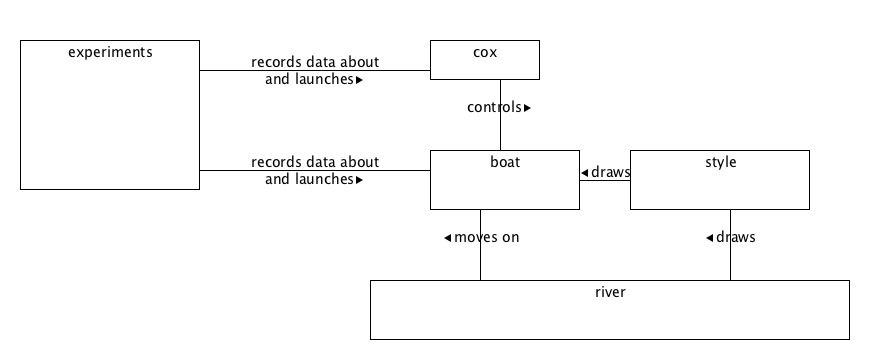
\includegraphics[scale=0.3]{images/packages.png}
  \caption{Model Overview}
  \label{software:fig:modeloverview}
\end{center}
\end{figure}



\section{\texttt{river} package}
The \texttt{river} package contains the classes that represent the river from our model. Figure \ref{software:fig:riverUML} gives an overview of the most important methods in the classes and the relationships between the classes.

\begin{figure}
\begin{center}
  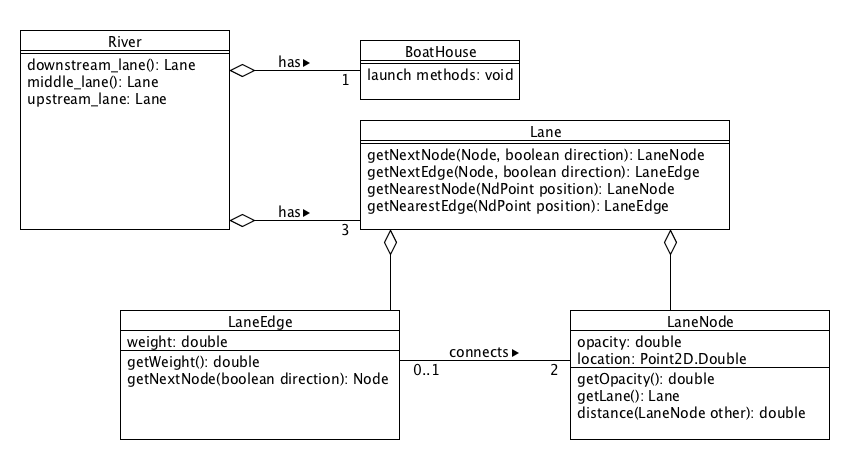
\includegraphics[scale=0.3]{images/riverpackage.png}
  \caption{Outline of the classes in the \texttt{river} package}
  \label{software:fig:riverUML}
\end{center}
\end{figure}

\subsection{River class}
The River is a container object. It holds the three lanes and the
boathouse. It is used to determine the relative positions of the lanes
(the lanes are stored in order in an array with the right-most lane when
heading downstream stored at the 0th index). The river overall
boundary for visualization purposes is defined by the boundaries of
the lanes. The river's top boundary is the bottom boundary of
the bottom lane and the it's top boundary is the top boundary
of the top lane. These boundaries are joined at each end to
complete the river.

\subsection{Lane class}

The lanes holds a network of nodes and edges using a Network
projection provided by Repast (see
\ref{software:dependencies:repast:network}). The Lane class uses the
Network methods provided by Repast to create helper methods for
navigating and searching a lane's graph. There are for getting the
next node or edge from a given node depending on the direction of
travel (upstream or not). There are also methods for finding the
nearest node or edge based on a provided location . These are useful
for spinning and changing lanes when the boat briefly deviates from
following the pre-defined lanes.

A Lane also stores a list of points either side of the nodes. This
provides a boundary for the lane which the River class uses to define
its own boundary.

The Lane class also has methods for building up a lane. There is a
\texttt{start} method used to place the first node of a lane's
graph. There is an \texttt{extend} method to place the next node in
the lane and join them with a graph. The extend method takes the angle
the joining line between the last placed node and the next node to be
place should be make with the horizontal as an argument. The distance
between each node is defined by the \texttt{static} variable
\texttt{edge\_length}. This will also place points in the top and
bottom boundaries. These points are placed on the lane perpendicular
to the extension. They are defined to be a fixed distance away from
the node. This distance is defined by the \texttt{static} variable
\texttt{width}.

\paragraph{code listing for extend()}

\lstinputlisting[language=Java,caption={Lane\#extend method for building a lane},label={listing:software:lane:extend}]{code/Lane.java.report}
\subsection{LaneNode class}
A LaneNode is a very simple object. It has a position attribute and
distance method. It also has a reference back to the Lane object in
which it is contained.
\subsection{LaneEdge class}
The LaneEdge class extends the Repast class RepastEdge<T>. This is so
the Repast Network interface can be used. The weight of an LaneEdge is
set to be the distance between the source and destination
nodes. LaneEdges are always directed edges. When travelling downstream
a boat travels with the direction of the edges, when travelling
upstream a boat travels against the direction of the edges. Therefore
for a given direction every node has a single edge leading out of it.

\subsubsection{Crashing}

LaneEdge class also keeps track of the coxes currently occupying it
in an array with methods add or a remove a cox from this array. (For
legacy reasons coxes rather than boats are tracked. It would fit the
model better to track the boats but since there is a one-to-one
mapping between boats and coxes this has not caused problems and so
has not been updated.) When a
cox is added, if there is already a cox occupying the edge then a
Crash object is created and associated with edge (unless there is
already one there) and the Crash object is reset.

Figure \ref{software:fig:crashingUML} shows the classes and main methods involved in the software implementation of a crash.

\begin{figure}
\begin{center}
  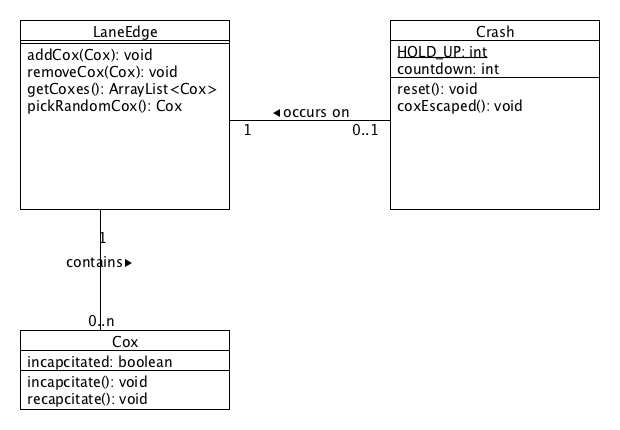
\includegraphics[scale=0.3]{images/crashing.png}
  \caption{Outline of the classes involved in a crash}
  \label{software:fig:crashingUML}
\end{center}
\end{figure}


When \texttt{reset()} is called on a Crash object, all the
\texttt{incapcitate()} method is called on all the coxes
occupying the edge associated with the Crash. This will prevent the
coxes from choosing and executing any actions. It will also bring the
cox's boat to an instant stop.

A count down then begins on the Crash object using a
ScheduledMethod. When the count down reaches zero, a cox is chosen at
random from the edge and this cox is allowed to carry out actions
again (by calling the \texttt{recapcitate()} method on it).

Each time a cox moves off the edge, another cox is chosen at
random and \texttt{recapcitate()} is called on it. This continues
until all coxes have moved off the edge or if a new boat moves onto
the edge, then the Crash is \texttt{reset} and the process starts
again from the beginning.

\subsection{LaneChangeEdge and TemporaryNode classes}\label{software:lane:lanechange}

The LaneChangeEdge class is an subclass of LaneEdge class. The
TemporaryNode class ian a subclass of LaneNode class. They are used
for the temporary graph branches that are created when a cox decides
to change lane.

TemporaryNode class is much the same LaneNode class except that
instances of TemporaryNode will respond \texttt{true} to the
\texttt{isTemporary()} method unlike
LaneNode. The same goes for LaneChangeEdge and LaneEdge classes. This
means it is possible to identify these temporary nodes and edges which
should be ignored by other boats.

LaneChangeEdge also holds the edge sandwiching LaneEdge objects from
the start and destination Lanes of the lane-change. When a cox is
added to or removed from a LaneChangeEdge, it is added to or removed
from these sandwiching LaneEdges. This means a boat effectively fills
two lanes when changing lanes.

LaneChangeEdge also has a \texttt{static} method called \texttt{createLaneChangeBranch}. It is used to creating this
set of TemporaryNode and LaneChangeEdge objects from the starting
point to the destination lane. It does this by finding the nearest
edge to the starting point in the starting and destination lane. The
first temporary node is placed at the starting point. The next node is
placed part way between the end nodes of the edges found. The process
is repeated using the next edges in the sandwiching lanes and placing
the temporary node slightly closer to the destination edge end
node. The process stops after a fixed number of loops when rather than
placing a temporary node, the actual node from the destination lane is
used.

\paragraph{LaneChageEdge build method code listing}

\subsection{Boathouse class}
\paragraph{The ``agent'' which contains the methods for launching a boat}
The BoatHouse class is a simple class. It has methods for launching
boats onto a River. The main launch method will create new Boat and
Cox objects, add them to the main context and then launch the objects
by placing them on the River by the boat house. It takes arguments to
allow the setting of desired gear, speed multiplier, distance to
cover and control policy to use as well as an id of a row in the
scheduled\_launches table to record data.

\subsection{RiverFactory class}
\paragraph{Helper class for creating pre-defined Rivers, adding them
  to context and positioning them appropriately in the Continuous
  Space projection, e.g. the simplified Cam. c.f. Factory pattern}
The RiverFactory class is a helper class with methods for easily creating
predefined River objects such as the simplified Cam. The factory will
define the appropriate angles to extend the River by as well as adding
the River and Boathouse to the context and placing them in the
Continuous Space projection in a suitable place.

\section{Boat package}
\paragraph{Opening paragraph and UML diagram}
The Boat package contains classes related to the model of a boat. It
consists of the main Boat class and a BoatNavigation class. Each Boat
has access to a BoatNavigation instance.

\subsection{Boat class}
The Boat class contains the properties about the boat such as current
orientation and gear, the speed multiplier. There are methods for
getting and, where appropriate, setting these properties. Boat objects are also the
objects that move around the Continuous Space projection and so the
Boat class contains methods for moving the boat in this
projection. The Boat object also holds a reference to a BoatRecord
object for collecting experimental data.

The scheduled method for Boat will call continueForward() on the
BoatNavigation instance and then update the BoatRecord's statistics.
\subsection{BoatNavigation class}
\paragraph{Keeping track of things like current edge and
directions of travel (upstream or downstream)}
BoatNavigation is a delegate class for Boat. It keeps track of the
boat's position on a Lane's network of nodes with references to the
current edge the boat is travelling on, the direction of travel
(stored as a boolean for upstream or not) and the amount of the edge
remaining before the next node. There are getter methods for
retrieving these properties as well as methods for getting related
information such as a the destination node that the Boat is currently
aiming at.

\paragraph{Keeping in sync location of cox and boat in 2D space and on the 1D lane graph}
The main continueForward() function takes care of keeping the
boat's movement within the 2D ContinuousSpace in sync with
movement on the 1D lane graph. As part of this it also takes care of
aiming the boat in a new direction each time it moves onto the next
edge.

\lstinputlisting[language=Java,caption={BoatNavigation\#continueForward
    method for moving a boat each tick},label={listing:software:boatnavigation:continueForward}]{code/BoatNavigation.report.java}

\section{Cox package}
\paragraph{Opening paragraph}
The main aim of the Cox package is to decide actions to execute in order to have the boat behave in a suitable manner. It therefore contains functionality for making observations, choosing an action based on those observations and executing the chosen action. Figure \ref{software:fig:coxUML} gives a UML sketch of the objects and their relationships in the package.

\begin{figure}
\begin{center}
  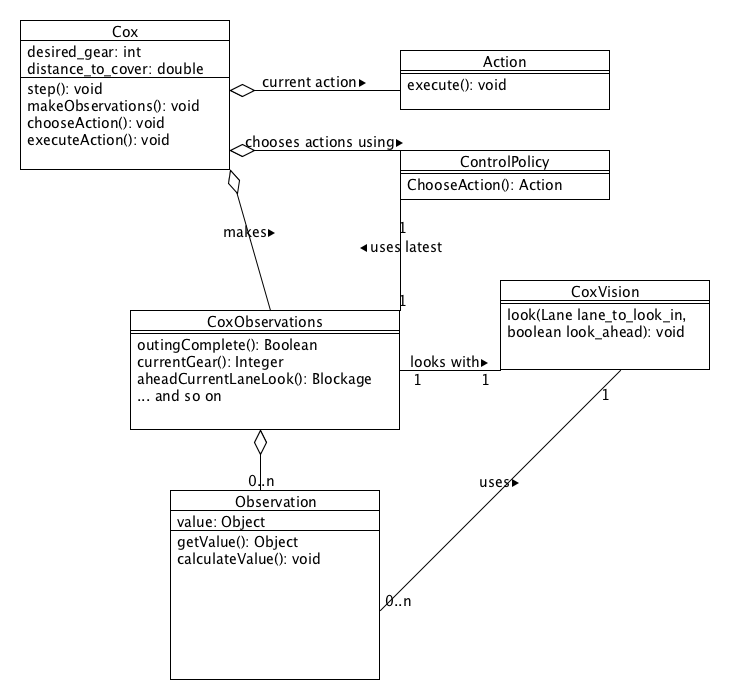
\includegraphics[scale=0.3]{images/coxpackageUML.png}
  \caption{Outline of the classes in the cox package}
  \label{software:fig:coxUML}
\end{center}
\end{figure}

\subsection{Cox class}
\paragraph{scheduling decision making}
The Cox class is the main class in the package. It is responsible for carrying out the 

\subsection{CoxObservations class}
\paragraph{how observations are made available to cox brain}
The CoxObservations class provides access to the many Observations a cox is allowed to make. It is designed to be consumed by a Control Policy. By wrapping the observations in a single class it provides a simple interface for a Control Policy to use when deciding what to do next. It also provides a way to restrict the Control Policy to only accessing information it is allowed based on the model rather than giving it access to raw Boat, River and Cox objects in the simulation.

The Observations that can return information in one of three types: simple booleans, integer values and Blockage objects, which are the result of looking down a lane. The information in the Blockage objects is inferred based on an instance of the CoxVision class. The CoxVision class provides methods for looking ahead and behind in each lane. An observation which makes use of this will return a Blockage object which will say for the fixed lane and direction, the number of edges until the blockage, whether the blockage is an edge occupied by boats or not, and the max and min relative speed of any boats on that blocked edge.

The observations are:
  \begin{itemize}
    \item{OutingOver} Returns true if the boat is back near the boathouse and has travelled the Cox's distance\_to\_cover value.
    \item{AtRiverEnd} Returns true if the boat is near the end of the river (either at the lock or the boathouse). Used so the cox knows to spin.
    \item{AboveDesiredSpeed and BelowDesiredSpeed} Return true if the boat's current gear is above or below the Cox's desired\_gear value. 
    \item{BoatGear} Returns the value of the boat's current gear (an integer).
    \item{AheadCurrentLane, BehindCurrentLane, AheadLeftLane, BehindLeftLane, AheadRightLane, BehindRightLane} : Returns the Blockage object based on looking in the appropriate direction and lane.
  \end{itemize}
  
\subsection{Control Policies}
  Each cox contains an instance of a ControlPolicy subclass. Each subclass will implement a different policy. A ControlPolicy class is updated each tick with the latest CoxObservations object. It uses these observations to decide what to do next.  Each control policy has a method called chooseAction(). This is defined in the superclass ControlPolicy so that all Control Policies have the same top-level goal condition which will check the OutingOver observation. If OutingOver determines the outing to be over then the Land action will be executed by the cox and the cox and boat will be removed from the simulation. Otherwise, a method called typeSpecificActionChoice() is executed. Each different control policy defines this differently. It is written in a teleo-reactive (TR) style for all Control Policies. This is done in Java by having a list of if statements. Each if statement will check a condition and if the condition is true, it will return the associated action. Otherwise it will move on to trying the next condition-action pair. The final if statement takes the constant true condition. This ensures one action will always be returned. The more complicated control policies contain nested TR-programs to make them easier to code and to read but they remain TR in style. The actual control policies tried are covered in the Chapter \ref{chapter:control_policy}
  
\subsection{Actions}
  Each action the cox can carry out has its own class. Every action provides a \texttt{typeSpecificExecute()} method. This method defines what happens when the cox executes the corresponding action. Since actions like spinning can carry on for more than one turn, this action returns true only when the action is complete. The abstract superclass \texttt{Action} defines the main \texttt{execute()} method. This checks the return value of \texttt{typeSpecificExecute()} and nullifies the Cox object's reference to current action, so that next turn the cox is free to choose again.

  There are 6 actions: LetBoatRun, Spin, SlowDown, SpeedUp, MoveToLaneOnLeft and MoveToLaneOnRight.
  
  LetBoatRun does nothing. The boat will continue to move forward in the same gear.
  
  Spin will turn the boat around and move it to the right hand lane over the course of 60 ticks. Because the movement of the boat during spinning is so different to the normal forward movement, the Spin instance itself calls methods on the Boat and BoatNavigation instances. When first executed the Spin action will work out the nearest node in the right hand lane (right relative to the cox when it starts). Each tick of execution the boat will rotate a small amount and move a little closer to the so that node so the boat appears to spin naturally in the visualization. During spinning the boat will occupy edges in all three lanes of the river. When spinning is complete, the boat is set to occupying the edge leading out of the node to which it spun (based on its new direction now it has spun).
  
  SpeedUp and SlowDown simply shift the boat's gear up or down one. If the boat is in the top gear or bottom gear, respectively, the action will have no affect so it will behave just like LetBoatRun.
  
  MoveToLaneOnLeft and MoveToLaneOnRight behave very similarly. The work out which lane the cox is trying to move to (so the lane on the cox's left or right respectively). It then creates a path of temporary edges and nodes using the LaneChageEdge class as described in \ref{software:lane:lanechange}. If the cox is already changing lanes, or there is no lane on the given side (e.g. try to move left when in the left-most lane) or there is not enough of the river left to fit in the lane change, then the action will silently fail and the action will behave just like LetBoatRun.

\section{Experiment package}\label{software:experiment}
The experiment package contains classes for gathering data each time a
simulation is run and storing the data in the database. The
InprogressSimulation class deals with setting and and finishing off
each simulation run, ensuring that all data is flushed to the
database. The BoatRecord and CrashRecord classes relate to particular
tables in the database, storing data related to each boat launched and
each crash. Care was taken to ensure that enough data was recorded
from each simulation run so that any experiments could be repeated.
The best way to examine this package is to look at the database schema.

\subsection{Database schema}\label{software:experiment:db}

The database schema is visualized in the Figure
\ref{software:fig:eer}. The \texttt{schedules}, \texttt{scheduled\_launches} and
\texttt{simulation\_parameters} tables are used for setting up simulation runs for an
experiment. The \texttt{simulation\_runs}, \texttt{boat\_records} and
\texttt{crash\_records} tables are used to hold data generated each
time the simulation is run.

\paragraph{ER diagram}

\begin{figure}
\begin{center}
  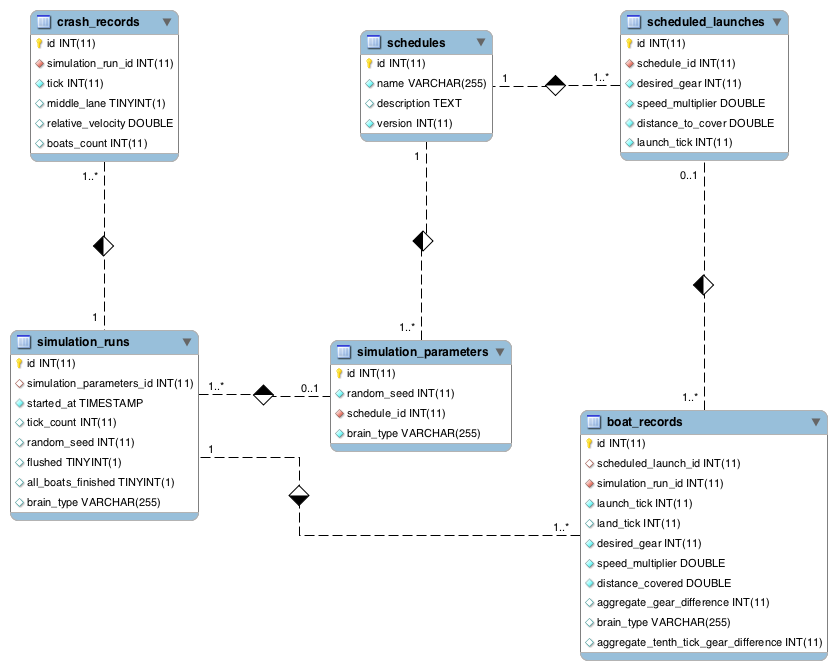
\includegraphics[scale=0.3]{images/eer.png}
  \caption{EER model of database}
  \label{software:fig:eer}
\end{center}
\end{figure}

\subsection{\texttt{simulation\_parameters}}
\texttt{simulation\_parameters} table holds information used to setup
an automated simulation run. These are the random seed, the control
policy and the schedule to use.

\subsection{\texttt{schedules} and \texttt{scheduled\_launches}
  tables}
The \texttt{schedules} and \texttt{scheduled\_launches} tables contain
information about pre-defined parameters for launching boats such as
during which tick the boat should be launched and what it's desired
gear should be.


\subsection{\texttt{simulation\_runs}}
The \texttt{simulation\_runs} table contains information about each
time the simulation is run. In the case it is an automated run,
simulation\_parameters\_id will contain the id of corresponding row in
texttt{simulation\_parameters table. it contains historic record of parameters
  used in the simulation are to ensure that experiments can be
  duplicated. These are the random seed and control policy used. It
  also stores how many ticks the simulation run lasted. There is also
  some useful metadata. This is the time the run started and whether
  all the data was successfully flushed to the database at the end (in
  case a of a crash). Further data about the simulation run is stored
  in the \texttt{boat\_records} and \texttt{crash\_records} tables.

\subsection{\texttt{boat\_records} and \texttt{crash\_records} tables}
The \texttt{boat\_records} table contains both historic records of the
boat's launch parameters and data about what happened to the boat
during the simulation.

\subsubsection{Launch parameters record}

\begin{itemize}
  \item{desired\_gear:} The gear the cox would ideally have the boat
    in.
  \item{brain\_type:} The name of the control policy used by the
    cox. This is the name of a Java class.
  \item{launch\_tick:} The tick during which the boat was launched.
  \item{speed\_multiplier:} The speed multiplier of the boat the cox
    is in.
  \item{scheduled\_launch\_id:} A link to the row in the
    \texttt{scheduled\_launches} table when the launch is part of an
    automated schedule.
  \item{simulation\_run\_id:} A link to the simulation run during
    which this boat was launched.
\end{itemize}

\subsubsection{What happened}
\begin{itemize}
  \item{land\_tick:} The tick when the boat landed. If the boat dails
    to land, this will be NULL.
  \item{distance\_covered:} The distance covered by the boat in the
    course of the simulation.
  \item{aggregate\_gear\_difference:} At each tick, the absolute
    difference between the boat's current gear and the cox's desired
    gear is calculated. This column contains the sum of these values.
  \item{aggregate\_tenth\_tick\_gear\_difference:} As above but the
    gear difference is only recorded every tenth tick. Recording every
    tick may turn out to be too excessive. This column is useful to
    hide short-lived, infrequent variations in gear.
\end{itemize}

The \texttt{crash\_records} table contains data for each pair of boats that crash during a simulation run. When a boat occupies an edge with boats already on, then it is considered to have crashed with all those boats and creates a new row in \texttt{crash\_records} for each. Each row of data consists of the relative velocity of the crash, the number of boats on the edge where the crash occurred, and whether this edge is in the middle lane of the river.

\section{Style and UI packages}
The style and ui packages are both small. They are used to customise the Repast
GUI. 

The style package contain classes
that define how to draw the River, Boathouse and Boat objects on the
screen. Repast provides some default stylings for objects. These style
classes are used to customise the appearance of objects more finely,
such as the boat shape or displaying the river.
Repast's StyleOGL2D interface. Settings in the XML config are used to
connect agent types to style classes. The style classes are then
interogated by Repast when drawing object each tick.

The ui package contains a single class, UserPanel. A simple JPanel which
can be added to Repast's interface and be used in to provide manual
controls. UserPanel contains buttons to launch coxes with control
policies designed to demonstrate the actions available to it. This is
very helpful for debugging actions and boat movement.

\section{Future Work}
There is still room for improvements in the software. These are outlined in this section.

\subsection{Lane Changing}
The changing lane implementation currently prevents a cox from changing lanes again while midway between lanes. It is acceptable that when moving to the lane on the left, say, the cox should not be able to move to the lane two to the left. However, the code and the model would be improved by allowing a cox to move back to the starting lane midway through a change - effectively the cox realises he should not try and change lanes

\subsection{Interactive Mode}
There is an interactive mode in the application that allows the user to launch boats by hand. Currently this is just for launching test boats that demonstrate the actions available to the cox. This could be improved by also allowing the user to choose the actions for a boat. The visualization could be changed to give a cox's eye view so that the simulation could also be used for training new coxes.

\subsection{Code tidy up so that it matches the model more closely}
There are a couple of places in the code which do not so obviously match up to the model. Neither are not essential fixes and do not cause the code to violate the model. However, it would be nice to change these so the code is a little more readable. 

The Boat Navigation object is referenced from the Cox class, when in fact this class is tied to keeping boat movement on the lanes and in the 2D space in sync. It would be nice to move this reference to the Boat class.

Secondly, a LaneEdge object keeps track of the Cox objects that currently occupy it. The code would match the model much more directly if instead it kept track of Boat objects.

\subsection{Optimized observation code so policies can have a memory}
Finally, there the observation code could be optimized. At one point I tried to have the cox's observations frozen each tick so that each CoxObservation object would return the same value during later ticks. This would then allow a cox to build up a sort of memory by storing these observations, which might allow some interesting new control policies.


This ends the description of the software behind the simulation and some possible future improvements. Appendix \ref{appendix:user_guide} also gives some more detail, especially on how to get the application running. Hopefully this chapter gives enough of an introduction to the software that any further questions can be answered by looking in the source code.
